\chapter{Kommunikation}\label{ch:communication}
Som nævnt i sektion \ref{sec:distSys} foregår kommunikationen i flere lag, herunder frontend (præsentationslag), logik lag som tilgås gennem QWest.API, og et datalag som er databasen, der tilgås af QWest.DataAccess. 
Når programmet startes de forskellige services nævnt i sektion \ref{sec:servicesArc}. QWest.Web oprettes som en proxy der sender HTTP Requests \cite{DistributedSystems}, og hele opstartsprocessen kan ses på figur \ref{fig:startup_log}.

\begin{figure}
    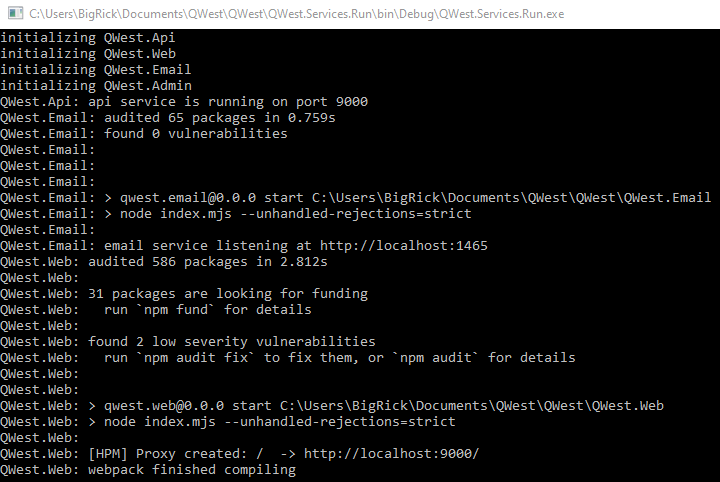
\includegraphics[width=\linewidth]{services_run_log.png}
    \caption{QWest.Services.Run opstarts log.}
    \label{fig:startup_log}
\end{figure}

Bruger-klienten tilgås gennem en browser, som sender HTTP Requests til \texttt{QWest.API}, der så kalder controllers til DAO til databasen. Som nævnt i sektion \ref{sec:REST} bruges der Json.NET til serialisering og JSON data til deserialisering. Da projektet er gennemført med REST, er der ingen konstant forbindelse til databasen, men i stedet laves der kun forbindelser når databasen skal opdateres ud fra en brugeroperation. 

\section{Sikkerhed}\label{sec:security}
HTTPS vil være den primære måde at sikre os, at bruger input er sikkert krypteret mens de bliver transporeret til QWest.Api, .NET framework skulle have support for HTTPS. \cite{DotNetFrameworkSSL} Der er ikke lagt arbejde i at sætte dette op, eftersom vi ikke ejer it SSL certificate. 
Måden autentificering er implementeret i systemet, er gennem login siden. Man skal være logget ind som bruger med brugernavn og password, for at kunne tilgå andre dele af systemet. Hver file-path som kan tilgås på hjemmesiden, checker om det er den korrekte bruger der er logget ind. Hvis ikke, så sendes brugeren til forsiden, hvor de kan logge ind eller oprette bruger.
For at sikre vores brugere mod leaking af deres passwords, såfremt der sker et data breach, hasher og salter vi alle brugeres passwords. Der bruges \texttt{Rfc2898DeriveBytes} \cite{Rfc2898DeriveBytes} til dette. Denne klasse bruger SHA1, som ikke er en optimal sikker hashing metode, hvilket burde ændres i næste iteration af projektet \cite{HowsecureisSHA1} til BCrypt \cite{BCrypt} eller lignende.

Når data skal lagres i databasen, bruges der SQL parametre for at undgå SQL injections. Som det kan ses i kodestykket \ref{lst:SQLinjection}, så bruges der en parametriseret SQL query string, hvor argumenterne metoden tager imod, placeres i de tilsvarende SQL parametre.

\begin{listing}[p]
    \begin{minted}
    [
        frame=lines,
        framesep=2mm,
        baselinestretch=1.2,
        bgcolor=LightGray,
        fontsize=\footnotesize,
        linenos,
        breaklines
    ]{csharp}
public async Task Update(Post post) {
    if (post.Id == null) {
        throw new ArgumentException("Editing a post needs a post ID");
    }
    string query = @"
UPDATE posts
SET content = @content
WHERE id = @post_id";
    await _conn.Use(query, async stmt => {
        stmt.Parameters.AddWithValue("@content", post.Contents);
        stmt.Parameters.AddWithValue("@post_id", post.Id);
        await stmt.ExecuteNonQueryAsync();
        return true;
    });
}
\end{minted}
\caption{QWest.DataAccess.Mssql.PostImpl\label{lst:SQLinjection}}
\end{listing}

\section{Transactions}\label{sec:transactions}
% Transactions
% Identify places in the application where we need transactions
% How do we build our transactions? Isolation levels?
% Do we need distributed transactions?
% ACID, Parallelism, Async/Await,
% Implementation details welcome
% Transactions and distributed systems from \cite{DistributedSystems}
En SQL Transaction \cite{sqltransactions} består af en række operationer, hvor enten alle sammen skal kunne eksekveres eller også skal ingen af dem eksekveres. Det klassiske eksempel hvor dette er nødvendigt er bank-transaktioner, hvor en person sender penge til en anden person. I dette scenarie vil pengene blive trukket fra kontoen på personen der sender pengene og lagt til modtagerens konto. Dette udføres af 2 operationer, så hvis databasen bliver utilgængelig når den første operation er udført men ikke den anden operation, så er pengene forsvundet fra databasen. Hvis operationerne skete i omvendt rækkefølge ville pengene blive sat ind på en konto, men ikke komme nogle steder fra. 

Løsningen på dette eksempel er SQL Transactions. SQL Transactions sørger for, at alle operationer, der sker i transaktionen, er afhængige af hinanden, sådan at enten vil hele transaktionen blive udført eller også bliver intet udført. I denne kontekst er der nogle krav der kan overholdes. ACID, som er et akronym der står for, Atomicity, Consistency, Isolation og Durability, beskriver en række krav, som omhandler fire hovedegenskaber en transaktion har. \cite{acid}

\subsection{ACID: Atomicity}\label{sec:acidAtomic}
Atomicity betyder at transaction'en ikke kan splittes op i mindre dele. En transaction er et individuelt "unit of work" og skal være alt eller intet. \cite{DistributedSystems} I bank eksemplet er dette meget relevant, det det har indflydelse på at penge ikke forsvinder eller bliver skabt ud af ingenting. 

Dette betyder også, at der aldrig er tidspunkt, hvor den første operation er skrevet til databasen, men anden operation ikke har. Der er kun én aktion.

\subsection{ACID: Consistency}\label{sec:acidConsistent}
Consistency betyder at reglerne sat op i SQL databasen (såsom \textit{unique constraints}, \textit{not null constraints} og \textit{foreign keys} \cite{SqlConstraints}) skal overholdes. Det vil sige at værdien der skal ændres skal være samme værdi fra start til slut af transaktionen.

\subsection{ACID: Isolation}\label{sec:acidIsolated}
Isolation betyder at SQL Transactions ikke skal være afhængige af andre SQL Transactions.

\subsection{ACID: Durability}\label{sec:acidDurable}
Durability betyder at når SQL transaktionen er fuldført, så skal der være persistens på den data, som er blevet opdateret/slettet/indsat.

\subsection{Transaction'er i QWest}\label{sec:transactionQwest}
I QWest.DataAccess.ConnectionWrapper findes hjælpemetoden \texttt{Use} \ref{lst:connectionWrapperUse}. Denne metode åbner en forbindelse til databasen, og starter en \texttt{SQLCommand} baseret på det første argument i metoden; en SQL query. En \texttt{SQLCommand} er som udgangspunkt en del af en transaktion, lige meget hvor mange queries der er i query-strengen. Det andet argument er en funktion, givet af metoden som kaldes, der bliver eksekveret med en \texttt{SQLComamnd}. Så snart den er fuldført lukkes forbindelsen. Et eksempel på brugen af Use-metoden kan findes i \texttt{Update(Post post)} metoden for \texttt{QWest.DataAccess.DAOPost} på kodelisten \ref{lst:SQLinjection}. Inde i scopet af funktionen givet til Use-metoden er forbindelsen åben. Så snart programmet kommer udenfor scope lukkes forbindelsen.

\begin{listing}[p]
    \begin{minted}
    [
        frame=lines,
        framesep=2mm,
        baselinestretch=1.2,
        bgcolor=LightGray,
        fontsize=\footnotesize,
        linenos,
        breaklines
    ]{csharp}
public async Task<T> Use<T>(string query, Func<SqlCommand, Task<T>> func) {
    var conn = Connection;
    conn.Open();
    T result = await func(conn.CreateCommand(query));
    conn.Close();
    return result;
}
\end{minted}
    \caption{QWest.DataAcess.ConnectionWrapper.Use\label{lst:connectionWrapperUse}}
\end{listing}

\section{Protokoller}\label{sec:protocols}
Kommunikationen mellem alle services i QWest er HTTP-requests, med untagelse af kommunikationen med databasen fra \texttt{QWest.DataAccess}. Kommunikationen fra frontend web klienten til \texttt{QWest.Api} (enten direkte eller med proxy gennem \texttt{QWest.Web}) skal selvfølgelig være HTTP, eftersom der ikke er nogle webstandarder for andre muligheder. Den eneste untagelse er WebSockets, men dette projekt har ikke en god Use Case\cite{Larman2004} for at bruge WebSockets og WebSockets har ikke lige så godt support blandt ældre browsere. Den implementerede kommunikation bruger igen JSON, eftersom frontend Javascript i browseren ikke understøtter mange andre måder at serialisere og deserialisere data på.

Der kan argumenteres for brug af en anden type kommunikation til og fra \texttt{QWest.Email}, eksempelvis har node.js muligheden for rå TCP og UDP, og en serializerings metode som ProtoBuf \cite{ProtoBuf} eller binær serialisering \cite{CsharpBinarySerialization}. Den unødvendige kompleksitet ville introducere tredjepartsbiblioteker i enten \texttt{QWest.Email} eller andre services som bruger \texttt{QWest.Email}, hvilket er grunden til at \texttt{QWest.Email} ender med at følge standarden ud fra kravene sat af \texttt{QWest.Api}, og bruger standard HTTP requests, der sender JSON serialiseret data.

\section{Caching and HTTP optimization}\label{sec:caching}
For at optimere systemet bruger vi caching. Caching er en teknik, hvor der lagres en kopi af en given ressource, som returneres ved forespørgsel. \cite{HTTPcaching} Dette bruges som regel til at gemme et resultat af en dyr operation, så man slipper for at gentage operationen. Det har fordelen at det reducerer mængden af beregninger, der skal laves, dog kan det kun implementeres de steder, hvor data ikke behøver at blive opdateret ofte eller steder hvor man ved at resultatet af operationen altid vil være den samme. 
Et eksempel på det første kriterie kunne være en informationsskærm, som fortæller gæster hvordan vejret er. Koden bag denne behøver ikke konstant at spørge eksempelvis DMI's API efter hvordan vejret er - en forespørgsel hver time ville være fint i de fleste tilfælde. Et eksempel på det andet kriterie kunne være \texttt{QWest.Web} servicen, som returnerer statiske filer, hvor der ikke er nogen grund til at læse data fra filsystemet, hver eneste gang, der bliver lavet en forespørgsel, såfremt filen allerede findes i hukommelsen.

HTTP protokollen har også indbygget caching \cite{HTTPcaching}, oftest i form af en \texttt{Cache-Control header}, der tillader en webserver at fortælle en browser, hvor lang tid resultater er cached for en specifik URL. I QWest bruges HTTP caching i projektets REST API - \texttt{QWest.Api} - når billeder bliver leveret, eftersom systemet er designet sådan, at det ikke tillader billeder at ændre sig. Dette betyder at flere end én HTTP request til \texttt{/api/Image/Get/<image\_id>} ville være overflødigt, og vi kan derfor bede browseren om at gemme resultatet (som i dette tilfælde er billedet) til næste gang billedet skal bruges, eksempelvis når man tilgår sin bruger profil. Cache tiden er på nuværende tidspunkt sat til 8765 timer (ca. ét år), eftersom \texttt{Cache-Control immutable} ikke er implementeret i alle browserer endnu.

\section{Middleware}\label{sec:middleware}
\texttt{QWest.Web} bruger Owin \cite{Owin} til at levere vores middleware. Det eneste middleware, der er skrevet manuelt, er \texttt{QWest.Api.AuthenticationMiddleware} klassen. Den undersøger om der er en autentificerings-token med i forespørgslen. Hvis der er, henter den brugeren som den autentificerings-token refererer til og lægger den i OwinContext. 